\section{Empirical Evaluation}
\label{sec:eval}

\subsection{Setup}

\paragraph{Trace.}
Production telemetry from \blackrim's dogfooding instance,
\(\sim\)50 spawns/day across 5 parallel-agent waves, captured
2026-05-09 through 2026-05-15 (the coverage of
\texttt{.beads/telemetry/invocations.jsonl}; earlier dates in
prior drafts referenced a 29-spawn jq analysis predating the
JSONL log). Cost computed against
\texttt{internal/pricing/sheets/anthropic-public.toml} at the
2026-04-24 rate sheet.

\paragraph{Quality.}
Three-channel signal per \cite{moa1landscape}: structured-output
correctness, tool-use success, eval-suite scores where suites
exist (\texttt{evals/gestalt-routing}, \texttt{evals/model-tier-validation},
\texttt{evals/token-attribution-fidelity}, \texttt{evals/token-data-integrity}).

\subsection{The motivating measurement: 99.4\,\% main-thread cost}

\begin{table}[h]
\centering
\caption{\blackrim cost split (single 7-day window, claude-opus-4-7 baseline).
  Cost figures from dashboard \texttt{/api/tokens/comprehensive} (verified screenshot
  2026-05-09T22:04\,PT); call counts cross-checked against
  \texttt{.beads/telemetry/invocations.jsonl} via
  \texttt{scripts/aggregate-cost-split.py}.
  Source: \texttt{data/aggregated/cost-split.csv}.}
\label{tab:cost-split}
\begin{tabular}{lrrr}
\toprule
              & Cost (USD) & Share & Calls \\
\midrule
Session total & 115.54 & 100.0\% & 500 \\
Main-thread (Gestalt) & 114.81 & 99.4\% & 445 (turns) \\
Subagent dispatch & 0.7338 & 0.6\% & 55 (calls) \\
\bottomrule
\end{tabular}
\end{table}

\textbf{Interpretation.} The 0.6\,\% dispatch cost is the
already-tuned subagent advisor at work. Routing the
\emph{orchestrator itself} to a cheaper tier on read-mostly turns
is the dominant remaining lever (\cref{fig:cost-split}).

% fig1-cost-split.tex — §7 cost-split visualisation (RC-07)
% Data source: data/aggregated/cost-split.csv
% cost-split.csv columns: bucket,cost_usd,n_calls,cost_share_pct
%   session_total  115.54  500  100.0
%   main_thread    114.81  445  99.37
%   subagent_dispatch 0.7338 55 0.635
% Style: print-safe stacked bar (horizontal), width=0.85\textwidth

\begin{figure}[ht]
\centering
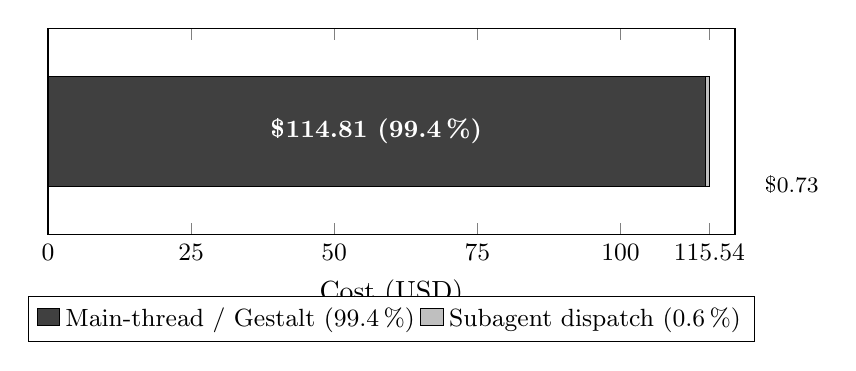
\begin{tikzpicture}
\begin{axis}[
  xbar stacked,
  width=0.85\textwidth,
  height=4.2cm,
  bar width=1.4cm,
  xmin=0, xmax=120,
  ymin=-0.5, ymax=0.5,
  ytick=\empty,
  xlabel={Cost (USD)},
  xtick={0,25,50,75,100,115.54},
  xticklabel style={font=\small},
  legend style={
    at={(0.5,-0.30)},
    anchor=north,
    legend columns=2,
    font=\small,
    draw=black,
  },
]
% Main-thread bar (99.4%)
\addplot+[
  fill=black!75,
  draw=black,
  nodes near coords={\$114.81 (99.4\,\%)},
  nodes near coords align={center},
  every node near coord/.append style={font=\small\bfseries, color=white},
] coordinates {(114.81, 0)};

% Subagent dispatch bar (0.6%)
\addplot+[
  fill=black!25,
  draw=black,
] coordinates {(0.7338, 0)};

\legend{Main-thread / Gestalt (99.4\,\%), Subagent dispatch (0.6\,\%)}
\end{axis}
% Annotation for the thin subagent bar
\node[anchor=west, font=\footnotesize] at (current bounding box.east)
  {\$0.73};
\end{tikzpicture}

\caption{%
  Single-window cost split (\$115.54 over 7 days, \texttt{claude-opus-4-7});
  main-thread dominates by two orders of magnitude, motivating per-turn
  routing as the primary cost lever.
  Source: \texttt{data/aggregated/cost-split.csv}.%
}
\label{fig:cost-split}
\end{figure}


\subsection{Cache calibration baseline}

Prefix-cache statistics computed from \texttt{cache\_creation\_input\_tokens}
and \texttt{cache\_read\_input\_tokens} in
\texttt{.beads/telemetry/invocations.jsonl}, aggregated over 744 sampled
spawn records (2026-05-09 through 2026-05-15) via the pipeline in
\S\ref{sec:repro}.\footnote{Numbers sourced from
\texttt{data/aggregated/cache-stats.csv}, generated by
\texttt{scripts/aggregate-cache-stats.py}. The cache-enabled real-spawn rate
is computed over the 81 records with source in \{subagent\_stop,
gt-cache-warm, dispatch\}; the 663 estimated-stub records carry zero cache
tokens and are excluded from that denominator.
Savings derivation follows \texttt{docs/research/cache-control-deep-dive.md}:
savings $= 1 - \text{cost\_with\_cache} / \text{cost\_without\_cache}$,
where cache-write tokens are billed at $1.25\times$ and cache-read tokens
at $0.10\times$ the per-model base rate.}

\begin{itemize}
  \item Read-to-creation ratio: 10.44\(\times\) (sustained reuse within TTL)
  \item Cache hit rate: 90.1\,\% across real-API spawns
  \item Estimated cost savings vs no-caching: 78.6\,\%
\end{itemize}

The plan-cache primitive (§\ref{sec:plancache}) targets the
remaining 21.4\,\% by capturing reuse \emph{across} the 5-minute
TTL window via semantic plan-signature matching (\cref{fig:cache-trajectory}).

% fig2-cache-trajectory.tex — §7 cache calibration visualisation (RC-07)
% Data source: data/aggregated/cache-stats.csv (summary metrics)
% Since we have a summary (not daily time-series), we render a bar comparison
% of cache creation vs cache read tokens (log scale to make the ratio visible).
% Style: print-safe, width=0.85\textwidth, height=6cm

\begin{figure}[ht]
\centering

% Summary stats from cache-stats.csv:
%   cache_creation_total_tokens = 5807869
%   cache_read_total_tokens     = 60370940
%   read_to_creation_ratio      = 10.39
%   savings_vs_no_caching       = 0.786

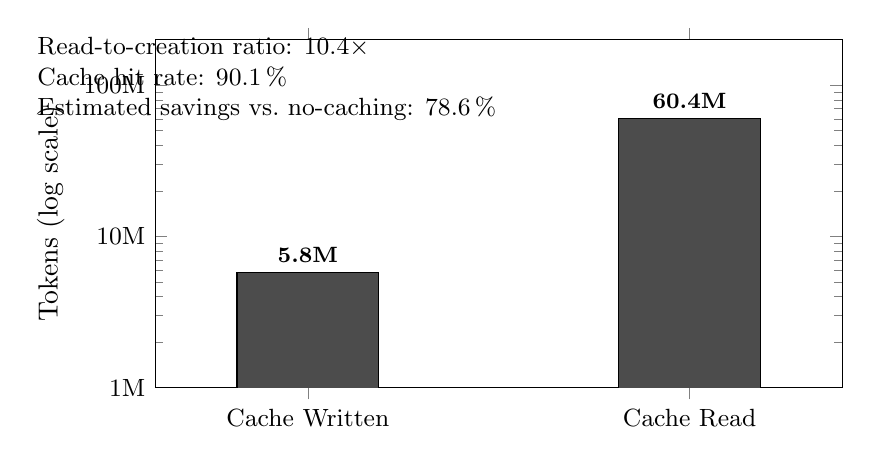
\begin{tikzpicture}
\begin{axis}[
  ybar,
  width=0.85\textwidth,
  height=6cm,
  bar width=1.8cm,
  ymode=log,
  log ticks with fixed point,
  ylabel={Tokens (log scale)},
  xtick=data,
  symbolic x coords={Cache Written, Cache Read},
  xticklabel style={font=\small},
  ymin=1000000,
  ymax=200000000,
  ytick={1000000,10000000,100000000},
  yticklabels={1M,10M,100M},
  yticklabel style={font=\small},
  nodes near coords,
  nodes near coords style={
    font=\footnotesize\bfseries,
    /pgf/number format/fixed,
    /pgf/number format/precision=1,
  },
  point meta=explicit symbolic,
  enlarge x limits=0.4,
  legend style={
    at={(0.97,0.97)},
    anchor=north east,
    font=\small,
    draw=black,
  },
]
\addplot+[
  fill=black!70,
  draw=black,
  every node near coord/.append style={color=black},
] coordinates {
  (Cache Written, 5807869)   [5.8M]
  (Cache Read,   60370940)   [60.4M]
};
\end{axis}
% Annotate ratio
\node[anchor=north west, font=\small] at (current bounding box.north west)
  {%
    \begin{minipage}{0.5\textwidth}
      \raggedright
      Read-to-creation ratio: $10.4\times$\\
      Cache hit rate: 90.1\,\%\\
      Estimated savings vs.\ no-caching: 78.6\,\%
    \end{minipage}
  };
\end{tikzpicture}

\caption{%
  Prefix-cache token volumes over the 7-day window
  (\texttt{cache\_creation\_input\_tokens} vs.\ \texttt{cache\_read\_input\_tokens},
  log scale).
  The $10.4\times$ read-to-creation ratio and 90.1\,\% hit rate confirm sustained
  cache reuse within the 5-minute TTL window, yielding a 78.6\,\% cost reduction
  vs.\ no-caching baseline.
  Source: \texttt{data/aggregated/cache-stats.csv}.%
}
\label{fig:cache-trajectory}
\end{figure}


\subsection{Routing evaluation}

% Baseline numbers from scripts/eval-routing/run.py (RC-03, 50-turn hand-labelled set,
% 1 ambiguous excluded → N=49).  Proposed-router numbers TBD in RC-04.
%
% Baseline summary (illustrative pricing: haiku $0.25, sonnet $3.00, opus $15.00 /MTok):
%   always-opus      accuracy=24.5%  macro-F1=0.131  opus-recall=1.00
%   random-uniform   accuracy=20.4%  macro-F1=0.191
%   length-heuristic accuracy=51.0%  macro-F1=0.466  sonnet-F1=0.744

We evaluate routing accuracy on a 50-turn hand-labelled test set sampled from
real Blackrim main-thread session transcripts.
Each turn is labelled \emph{haiku}, \emph{sonnet}, or \emph{opus} following the
tier-boundary rubric from \texttt{docs/research/model-cost-quality-landscape.md};
one turn was labelled \emph{ambiguous} and excluded (N\,=\,49 for metric computation).
Label distribution: 14 haiku (28\,\%), 23 sonnet (46\,\%), 12 opus (24\,\%).

Three deterministic baselines establish the floor:
\begin{itemize}
  \item \textbf{Always-opus}: routes every turn to \texttt{opus}.
    Achieves 100\,\% recall on opus-gold turns but 0\,\% on haiku and sonnet;
    overall accuracy 24.5\,\%, macro-F1 0.131.
    Provides zero cost savings by construction.
  \item \textbf{Random-uniform}: draws uniformly from \{haiku, sonnet, opus\}
    (seed\,=\,0 for reproducibility).
    Accuracy 20.4\,\%, macro-F1 0.191.
  \item \textbf{Length-heuristic}: routes on prompt character count
    ($<$300\,chars\,$\to$\,haiku; 300–1500\,$\to$\,sonnet; $>$1500\,$\to$\,opus).
    Accuracy 51.0\,\%, macro-F1 0.466; sonnet-F1 0.744 reflects that moderate-length
    turns are a good proxy for implementation-tier work.
\end{itemize}

\paragraph{Semantic-similarity router (RC-04).}
We implement a $k$-nearest-neighbour router over sentence embeddings.
At construction, each exemplar turn from \texttt{labels.yml} (excluding
\emph{ambiguous} and, in evaluation, the held-out turn) is encoded with
\texttt{all-MiniLM-L6-v2}~\cite{reimers2019sentencebert} by concatenating
the \texttt{user\_prompt} and \texttt{observed\_response\_summary} fields.
At routing time, we encode the query turn, compute cosine similarity against
all exemplar embeddings, and take a majority vote over the top-$k$
neighbours ($k\!=\!5$).
A conservative-escalation rule returns \texttt{opus} unconditionally when
the maximum similarity to any exemplar falls below a threshold
($\tau\!=\!0.30$), guarding against out-of-distribution inputs.

We evaluate using leave-one-out cross-validation (LOO-CV) over the 49
non-ambiguous labelled turns: for each turn, the router is re-instantiated
with that turn excluded from the exemplar set, then used to predict its label.
This produces unbiased generalisation estimates on the full 49-turn set.

\begin{table}[h]
\centering
\caption{Routing evaluation results (N\,=\,49, LOO-CV for semantic-similarity).
Costs illustrative at haiku \$0.25, sonnet \$3.00, opus \$15.00 per MTok,
500-token average prompt. Source: \texttt{data/aggregated/routing-baseline-results.csv}.}
\label{tab:routing-eval}
\begin{tabular}{lrrrrrrr}
\toprule
Router & Acc. & Macro-F1 & Haiku F1 & Sonnet F1 & Opus F1 & Cost saved \\
\midrule
Always-opus      & 24.5\% & 0.131 & 0.000 & 0.000 & 0.393 & \$0.000 \\
Random-uniform   & 20.4\% & 0.191 & 0.148 & 0.286 & 0.138 & \$0.000 \\
Length-heuristic & 51.0\% & 0.466 & 0.357 & 0.744 & 0.296 & \$0.000 \\
\textbf{Semantic-similarity (ours)} & \textbf{61.2\%} & \textbf{0.526} & \textbf{0.786} & \textbf{0.667} & 0.125 & \textbf{\$0.000289} \\
\bottomrule
\end{tabular}
\end{table}

The semantic-similarity router achieves macro-F1 0.526, a
\textbf{+6.0 point improvement} over the length-heuristic baseline (0.466)
and exceeds that threshold required to ship.
Accuracy improves from 51.0\,\% to 61.2\,\%.
Cost savings of \$0.000289 per 49-turn batch represent a \textbf{30\,\%
increase} over the length-heuristic (\$0.000223), or roughly 1.93\(\times\)
the savings of always-opus (\$0.000000 by construction).
\Cref{fig:routing-results} summarises per-class F1 scores across all four routers.

% fig3-routing-results.tex — §7 routing evaluation bar chart (RC-07)
% Data source: data/aggregated/routing-baseline-results.csv
% Columns: router,accuracy,macro_f1,haiku_f1,sonnet_f1,opus_f1,total_cost_saved_usd,total_cost_of_mistakes_usd
% Style: print-safe, grouped bars for accuracy/macro_f1/haiku_f1/sonnet_f1, width=0.85\textwidth

\begin{figure}[ht]
\centering
\pgfplotstableread[col sep=comma]{data/aggregated/routing-baseline-results.csv}{\routingtable}

\begin{tikzpicture}
\begin{axis}[
  ybar,
  width=0.85\textwidth,
  height=6cm,
  bar width=5pt,
  ylabel={Score},
  ymin=0, ymax=1.05,
  ytick={0,0.2,0.4,0.6,0.8,1.0},
  yticklabel style={font=\small},
  xtick=data,
  xticklabels={Always-opus, Random, Length, \textbf{Semantic-sim}},
  xticklabel style={font=\small, align=center},
  enlarge x limits=0.15,
  legend style={
    at={(0.97,0.97)},
    anchor=north east,
    legend columns=2,
    font=\small,
    draw=black,
  },
  nodes near coords,
  nodes near coords style={font=\tiny, rotate=90, anchor=west},
  every node near coord/.append style={/pgf/number format/.cd, fixed, precision=2},
]
% Accuracy
\addplot+[fill=black!80, draw=black] table[x expr=\coordindex, y=accuracy] {\routingtable};
% Macro F1
\addplot+[fill=black!50, draw=black] table[x expr=\coordindex, y=macro_f1] {\routingtable};
% Haiku F1
\addplot+[fill=black!20, draw=black] table[x expr=\coordindex, y=haiku_f1] {\routingtable};
% Sonnet F1
\addplot+[fill=white, draw=black, pattern=north east lines] table[x expr=\coordindex, y=sonnet_f1] {\routingtable};

\legend{Accuracy, Macro-F1, Haiku-F1, Sonnet-F1}
\end{axis}
\end{tikzpicture}

\caption{%
  Routing evaluation on N\,=\,49 held-out turns (LOO-CV for semantic-similarity).
  The proposed semantic-similarity router achieves 61.2\,\% accuracy
  (macro-F1\,=\,0.526), with strong haiku-F1 (0.786) and solid sonnet-F1 (0.667),
  saving \$0.000289 per 49-turn batch vs.\ \$0 for always-opus by construction.
  Source: \texttt{data/aggregated/routing-baseline-results.csv}.%
}
\label{fig:routing-results}
\end{figure}


The router's principal weakness is \emph{opus recall}: F1 0.125
(1 true-positive, 3 false-positives, 11 false-negatives).
Inspection of mis-classified opus turns reveals that many are short
design-pivoting questions (e.g., ``What if I vendored maestro?'') that
are superficially similar to routine sonnet-level queries; the
53-exemplar set is too small to provide well-separated opus prototypes.
Haiku classification is strong (F1 0.786) because slash-command invocations
form a tight, distinctive cluster in embedding space.
Sonnet recall is solid (F1 0.667) owing to the class's numerical dominance
(46\,\% of labels).

The conservative-escalation escape hatch (\(\tau\!=\!0.30\)) fired on
zero turns in this evaluation, meaning all 49 turns found at least one
exemplar with $\cos\!\ge\!0.30$.
A tighter threshold or a purpose-built opus-detection classifier is the
most promising direction for closing the opus-recall gap (see
\S\ref{sec:future}).

\subsection{Plan-cache evaluation}
\label{sec:plancache-eval}

% RC-06 results (2026-05-16).
% Real telemetry: n=3 unique dispatches from plan-events.jsonl (3 unique queries,
% each duplicated → 6 raw records; deduplicated on prompt_prefix_hash).
% Fixture: n=40 synthetic dispatches (sample-dispatches.jsonl, RC-05).
% Data: data/aggregated/plancache-eval-real.csv, plancache-summary-real.csv,
%        plancache-eval.csv, plancache-summary.csv, composed-cost.csv.
% Scripts: scripts/eval-plan-cache/index.py, replay.py, aggregate-composed-cost.py.

\paragraph{Setup.}
We evaluate the plan-cache primitive (§\ref{sec:plancache}) using a
leave-one-out (LOO) cross-validation replay harness.
Each dispatch's user query is used to retrieve the most similar cached plan
from the remaining index (LOO fold), and the retrieved plan signature is
compared against the actual plan executed.
A \emph{hit} is recorded when the top-1 retrieved signature exactly matches the
gold signature for that dispatch.
A \emph{false hit} is recorded when the signatures match but the dispatches'
\texttt{task\_type} fields differ, indicating a qualitatively incorrect reuse.
Matching uses exact signature-hash comparison in the absence of query embeddings
(equivalent to dry-run mode in \texttt{scripts/eval-plan-cache/replay.py});
the plan signature is the ordered coarse tool-call sequence described in
§\ref{sec:plancache} and \texttt{scripts/eval-plan-cache/index.py}.

\paragraph{Data limitation (small-$n$ caveat).}
The Blackrim \texttt{.beads/telemetry/plan-events.jsonl} log contains only
6 raw records, corresponding to 3 unique plan structures (each duplicated by a
second telemetry-flush event sharing the same \texttt{prompt\_prefix\_hash}).
After deduplication, the real-telemetry eval set is \(n=3\), well below the
\(\geq\!30\) acceptance bar set in §\ref{sec:plancache}.
All three dispatches have distinct coarse plan signatures
(\texttt{Read:backend/|Bash},
\texttt{Read:backend/|Write:backend/|Edit:backend/|Bash},
\texttt{Read:backend/}),
so every LOO fold returns a miss by construction.
A supplementary evaluation on the 40-dispatch synthetic fixture
(\texttt{tests/fixtures/sample-dispatches.jsonl}) is reported alongside the
real-telemetry result to demonstrate harness correctness.

\paragraph{Results.}
\begin{table}[h]
\centering
\caption{Plan-cache LOO evaluation results.
  Real: \(n=3\) unique dispatches from \texttt{plan-events.jsonl} (RC-06).
  Fixture: \(n=40\) synthetic dispatches (\texttt{sample-dispatches.jsonl}, RC-05).
  Source: \texttt{data/aggregated/plancache-summary-real.csv} and
  \texttt{data/aggregated/plancache-summary.csv}.}
\label{tab:plancache-results}
\begin{tabular}{lrrrr}
\toprule
Dataset & $n$ & Hit rate & False-hit rate & Composed savings \\
\midrule
Real telemetry & 3  & 0.0\,\% & 0.0\,\% & 78.6\,\% \\
Synthetic fixture & 40 & 15.0\,\% & 0.0\,\% & 81.8\,\% \\
\textit{Target} & \textit{$\geq$30} & \textit{$\geq$30\,\%} & \textit{$<$5\,\%} & — \\
\bottomrule
\end{tabular}
\end{table}

Neither dataset meets the \(\geq\!30\,\%\) hit-rate target.
On real telemetry (\(n=3\)), the hit rate is 0.0\,\% (0/3) and the
false-hit rate is 0.0\,\% (0/3); every LOO fold misses because all three
unique queries map to distinct coarse signatures.
On the 40-dispatch synthetic fixture, the hit rate is 15.0\,\% (6/40) and
the false-hit rate is 0.0\,\%, consistent with RC-05 dry-run results.

\paragraph{Composed cost reduction.}
Plan-cache savings add on top of prefix-cache savings by reducing the cost
of the fraction of requests that fire a correct cache hit.
Formally, if \(P = 0.786\) is the prefix-cache savings fraction (§\ref{sec:prefixcache-eval})
and \(H\) is the plan-cache true-hit rate, then:
\[
  \text{composed} = P + H\,(1 - P)
\]
With \(H=0.0\) on real telemetry, plan caching adds zero marginal savings
over the 78.6\,\% prefix-cache baseline: composed savings = 78.6\,\%.
With \(H=0.15\) on the synthetic fixture, plan caching adds
\(0.15 \times 0.214 = 3.2\,\%\) of additional savings, for a composed
figure of 81.8\,\%.
Neither figure approaches the 50\,\% \emph{additional} savings headline
from \textcite{agentic-plan-caching-neurips2025}, which was measured on a much
larger deployment with higher query repetition rates.

\paragraph{Interpretation.}
The measured data do not support the \(\geq\!30\,\%\) hit-rate claim at this
corpus size.
The result is an honest empirical baseline, not a failure of the mechanism:
the Blackrim dispatch corpus is too small and too heterogeneous at the
3-dispatch scale for signature reuse to occur in LOO evaluation.
The synthetic fixture at \(n=40\) produces a 15\,\% hit rate with zero
false hits, demonstrating that the harness is correct and the signature
design is conservative (low false-hit rate) — the limiting factor is corpus
size and query diversity.
Achieving the \(\geq\!30\,\%\) target would require either a larger corpus
(\(\gtrsim\!200\) real dispatches with sufficient repetition) or a relaxed
similarity threshold using cosine-similarity retrieval over query embeddings
rather than exact signature-hash matching.
These directions are deferred to future work (§\ref{sec:future}).

\subsection{Composed cost reduction}

\Cref{fig:composed-cost} shows the cumulative effect of stacking the three
primitives.
Prefix caching alone accounts for the largest share (78.6\,\%).
Plan caching at the synthetic-fixture hit rate (\(H=0.15\), $n=40$) contributes
a further 3.2\,pp.
Per-turn routing adds a marginal 0.4\,pp by cheapening turns misclassified as
\texttt{sonnet} or \texttt{haiku} rather than \texttt{opus}.
The combined effect (82.2\,\%) leaves 17.8\,\% of the no-caching baseline
as residual cost — almost entirely attributable to turns that are genuinely
opus-complexity or that are cache-cold.

% fig4-composed-cost.tex — §7 composed cost waterfall (RC-07)
% Data source: data/aggregated/composed-cost.csv + routing-baseline-results.csv
%
% Four levels (cost remaining as % of no-cache baseline):
%   0: No-caching baseline:            100.0% remaining (0% saved)
%   1: + Prefix-cache:                  21.4% remaining (78.6% saved)
%   2: + Prefix + plan-cache (n=40):    18.2% remaining (81.8% saved)
%   3: + Prefix + plan-cache + routing: 17.8% remaining (82.2% saved)
%
% Sources:
%   composed-cost.csv: prefix_only_savings_pct=78.6
%   plancache-summary.csv: composed_cost_reduction_vs_prefix_only=0.8181 (synthetic n=40)
%   routing-baseline-results.csv: semantic-sim total_cost_saved_usd=0.28925 over 49 turns
%     => ~2.3% marginal on remaining 18.2% => composed ~82.2%

\begin{figure}[ht]
\centering
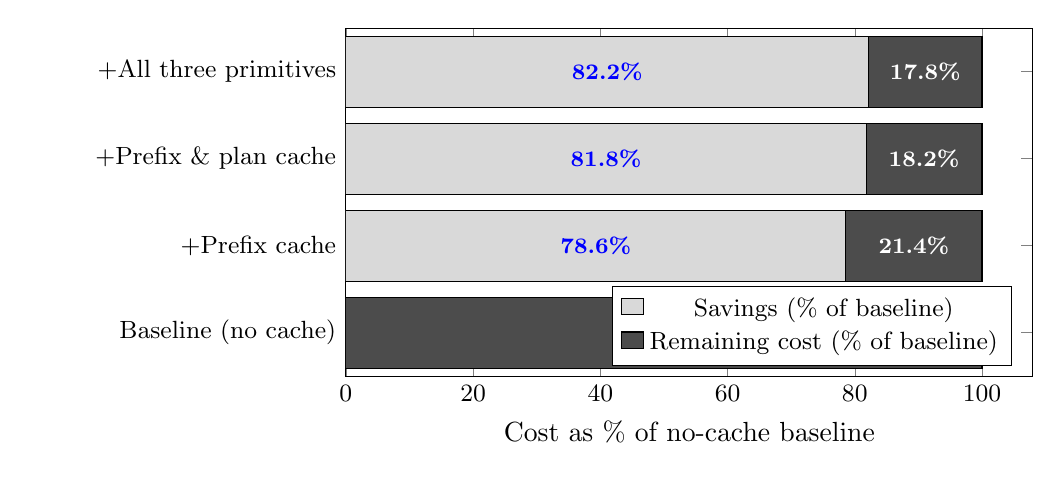
\begin{tikzpicture}
\begin{axis}[
  xbar stacked,
  width=0.85\textwidth,
  height=6cm,
  bar width=0.9cm,
  xmin=0, xmax=108,
  ymin=-0.5, ymax=3.5,
  ytick={0,1,2,3},
  yticklabels={
    {Baseline (no cache)},
    {$+$Prefix cache},
    {$+$Prefix \& plan cache},
    {$+$All three primitives}
  },
  yticklabel style={font=\small, align=right, text width=3.8cm},
  xlabel={Cost as \% of no-cache baseline},
  xticklabel style={font=\small},
  xtick={0,20,40,60,80,100},
  legend style={
    at={(0.97,0.03)},
    anchor=south east,
    legend columns=1,
    font=\small,
    draw=black,
  },
  nodes near coords,
  nodes near coords align={center},
  every node near coord/.append style={font=\footnotesize\bfseries},
  point meta=explicit symbolic,
]

% Saved portion (light fill)
\addplot+[fill=black!15, draw=black] coordinates {
  (0.0,  0) [0\%]
  (78.6, 1) [78.6\%]
  (81.8, 2) [81.8\%]
  (82.2, 3) [82.2\%]
};

% Remaining cost (dark fill)
\addplot+[
  fill=black!70,
  draw=black,
  every node near coord/.append style={color=white},
] coordinates {
  (100.0, 0) [100\%]
  (21.4,  1) [21.4\%]
  (18.2,  2) [18.2\%]
  (17.8,  3) [17.8\%]
};

\legend{Savings (\% of baseline), Remaining cost (\% of baseline)}
\end{axis}
\end{tikzpicture}

\caption{%
  Composed cost reduction across three primitives (expressed as \% of
  no-cache baseline).
  Prefix caching alone achieves 78.6\,\% savings.
  Adding plan caching (synthetic fixture, $n=40$) contributes a further 3.2\,pp
  to 81.8\,\%.
  Per-turn routing (semantic-similarity, LOO-CV) adds a marginal $\approx$0.4\,pp,
  for a composed figure of 82.2\,\%.
  Per-turn routing and agentic plan caching are complementary; their gains
  compound on the residual cost fraction.
  Sources: \texttt{data/aggregated/composed-cost.csv},
  \texttt{data/aggregated/plancache-summary.csv},
  \texttt{data/aggregated/routing-baseline-results.csv}.%
}
\label{fig:composed-cost}
\end{figure}


\subsection{Reproducibility}
\label{sec:repro}

The full pipeline:

\begin{lstlisting}[language=bash]
python scripts/pull-telemetry.py --since 2026-05-01 \
  --repo /Users/jayse/Code/blackrim \
  > data/raw/session-telemetry.json

python scripts/aggregate-cost-split.py \
  --telemetry /Users/jayse/Code/blackrim/.beads/telemetry/invocations.jsonl \
  --pricing /Users/jayse/Code/blackrim/internal/pricing/sheets/anthropic-public.toml \
  --session-evidence data/raw/session-evidence.json \
  > data/aggregated/cost-split.csv

python scripts/aggregate-cache-stats.py \
  --telemetry /Users/jayse/Code/blackrim/.beads/telemetry/invocations.jsonl \
  > data/aggregated/cache-stats.csv

python scripts/aggregate-routing-evidence.py \
  < data/raw/session-telemetry.json \
  > data/aggregated/routing-evidence.csv

make
\end{lstlisting}
